
%(BEGIN_QUESTION)
% Copyright 2010, Tony R. Kuphaldt, released under the Creative Commons Attribution License (v 1.0)
% This means you may do almost anything with this work of mine, so long as you give me proper credit

Dette ventilposisjoneringssystemet har et problem. Ventilen blir stående på 0\% (helt stengt) for {\it enhver} påtrykt reguleringssignalverdi:

$$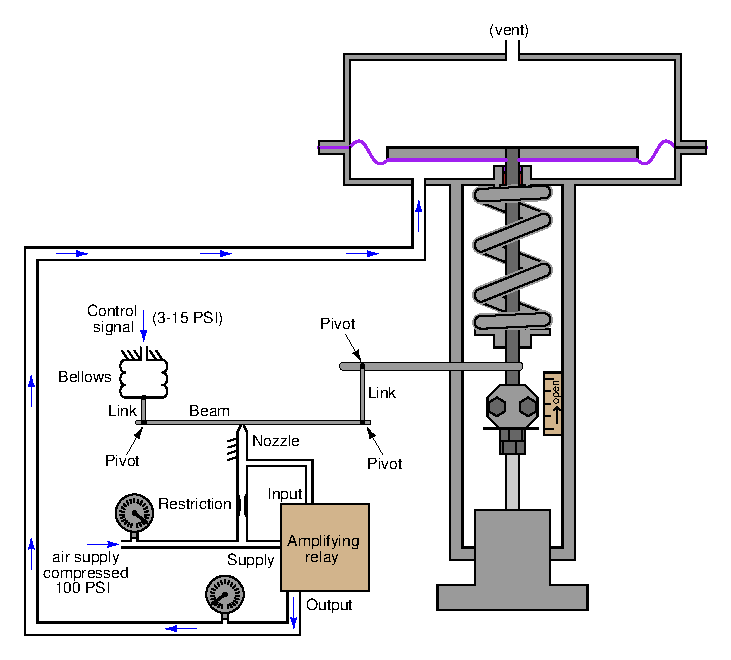
\includegraphics[width=15.5cm]{i01362x01.eps}$$

Når du ser på manometrene, legger du merke til at forsyningsmanometeret viser 75 PSI og utgangsmanometeret viser 0 PSI, samtidig som regulatorens utgang er satt til 100\% i manuell modus.

Vurder sannsynligheten for hver av de oppgitte feilene for denne ventilposisjoneren. Betrakt hver feil separat (dvs. ingen sammenfallende feil), og avgjør om hver enkelt feil alene kan forklare {\it alle} målinger og symptomer.

% Ingen blanklinjer er tillatt mellom linjer i en \halign-struktur!
% Jeg bruker kommentarer (%) i stedet, slik at TeX ikke feiler.

$$\vbox{\offinterlineskip
\halign{\strut
\vrule \quad\hfil # \ \hfil & 
\vrule \quad\hfil # \ \hfil & 
\vrule \quad\hfil # \ \hfil \vrule \cr
\noalign{\hrule}
%
% Første rad
{\bf Feil} & {\bf Mulig} & {\bf Umulig} \cr
%
\noalign{\hrule}
%
% Neste rad
Tettet restriksjon &  &  \cr
%
\noalign{\hrule}
%
% Neste rad
Tettet dyse &  &  \cr
%
\noalign{\hrule}
%
% Neste rad
Brudd i kobling til ventilspindel &  &  \cr
%
\noalign{\hrule}
%
% Neste rad
Lekkasje i belg &  &  \cr
%
\noalign{\hrule}
%
% Neste rad
Lekkasje i aktuatormembran &  &  \cr
%
\noalign{\hrule}
%
% Neste rad
I/P-utgang feilet lavt &  &  \cr
%
\noalign{\hrule}
%
% Neste rad
I/P-utgang feilet høyt &  &  \cr
%
\noalign{\hrule}
%
% Neste rad
Svikt i luftforsyning &  &  \cr
%
\noalign{\hrule}
} % Slutt på \halign
}$$ % Slutt på \vbox

Til slutt: angi den {\it neste} diagnostiske testen eller målingen du ville utført på dette systemet. Forklar hvordan resultatet/resultatene av denne testen hjelper videre med å identifisere plassering og/eller type feil.

\underbar{file i01362}
%(END_QUESTION)





%(BEGIN_ANSWER)

En god diagnostisk test her er å skyve klaffen mot dysen med fingeren for å se om ventilaktuatoren forsøker å åpne.

%(END_ANSWER)





%(BEGIN_NOTES)

% Ingen blanklinjer er tillatt mellom linjer i en \halign-struktur!
% Jeg bruker kommentarer (%) i stedet, slik at TeX ikke feiler.

$$\vbox{\offinterlineskip
\halign{\strut
\vrule \quad\hfil # \ \hfil & 
\vrule \quad\hfil # \ \hfil & 
\vrule \quad\hfil # \ \hfil \vrule \cr
\noalign{\hrule}
%
% Første rad
{\bf Feil} & {\bf Mulig} & {\bf Umulig} \cr
%
\noalign{\hrule}
%
% Neste rad
Tettet restriksjon & $\surd$ &  \cr
%
\noalign{\hrule}
%
% Neste rad
Tettet dyse &  & $\surd$ \cr
%
\noalign{\hrule}
%
% Neste rad
Brudd i kobling til ventilspindel & ? &  \cr
%
\noalign{\hrule}
%
% Neste rad
Lekkasje i belg & ? &  \cr
%
\noalign{\hrule}
%
% Neste rad
Lekkasje i aktuatormembran & ? &  \cr
%
\noalign{\hrule}
%
% Neste rad
I/P-utgang feilet lavt & $\surd$ &  \cr
%
\noalign{\hrule}
%
% Neste rad
I/P-utgang feilet høyt &  & $\surd$ \cr
%
\noalign{\hrule}
%
% Neste rad
Svikt i luftforsyning &  & $\surd$ \cr
%
\noalign{\hrule}
} % Slutt på \halign
}$$ % Slutt på \vbox

Feilen ``Brudd i kobling til ventilspindel'' er mulig bare dersom bjelken faller {\it bort} fra dysen og ikke mot den (det skjematiske bildet er ikke ment å antyde at dysen er {\it under} bjelken!). ``Lekkasje i aktuatormembran'' er bare mulig hvis lekkasjen er katastrofal, slik at det ikke kan bygges opp merkbart mottrykk til tross for at posisjoneren forsøker maksimalt å bygge trykk der. Det samme gjelder ``Lekkasje i belg'', som bare kan være korrekt hvis lekkasjen er så stor at belgen ikke kan ekspandere i det hele tatt.

\vskip 20pt \vbox{\hrule \hbox{\strut \vrule{} {\bf Virtuell feilsøking} \vrule} \hrule}

Dette spørsmålet egner seg godt som en ``virtuell feilsøking''-øvelse. Når du presenterer diagrammet for studentene, ser du først for deg en bestemt feil i systemet. Deretter presenterer du ett eller flere symptomer på denne feilen (noe en operatør eller annen bruker av systemet kan observere). Studentene foreslår så ulike diagnostiske tester som kan utføres for å identifisere feilens natur og plassering, som om de var teknikere som feilsøker problemet. Din oppgave er å fortelle hva resultatet/resultatene ville blitt for hver foreslåtte test, og dokumentere disse slik at alle studentene kan se dem.

Under og etter øvelsen er det nyttig å stille oppfølgingsspørsmål som:

\begin{itemize}
\item{} Hva forteller resultatet av den siste diagnostiske testen om feilen?
\item{} Anta at resultatet av den siste diagnostiske testen var annerledes. Hva ville det i så fall fortalt om feilen?
\item{} Er den siste diagnostiske testen den beste vi kunne gjort?
\item{} Hva ville vært den ideelle testrekkefølgen for å diagnostisere problemet med færrest mulig trinn?
\end{itemize}

\vfil \eject

\noindent
{\bf Oppsummeringsquiz:}

Identifiser virkningene av at restriksjonen tettes med partikler i denne ventilposisjoneringsmekanismen:

$$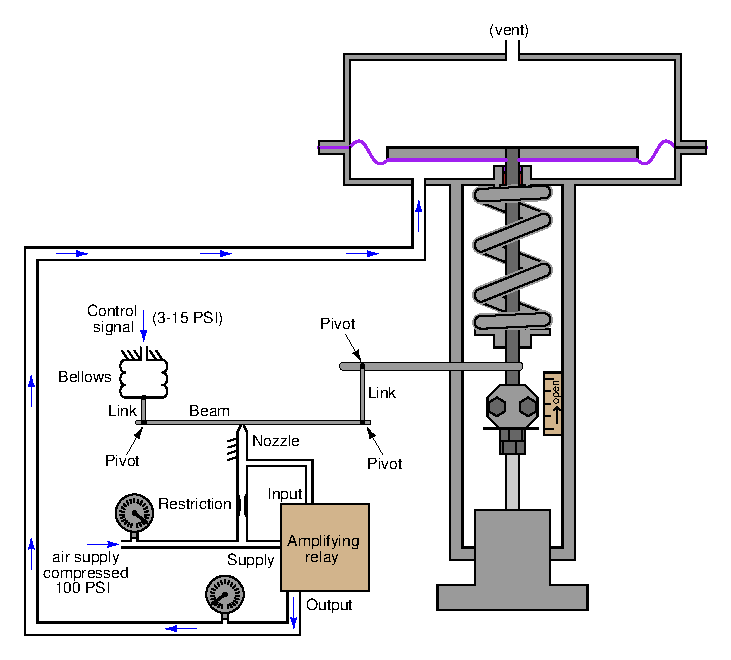
\includegraphics[width=15.5cm]{i01362x01.eps}$$

\begin{itemize}
\item{} Reguleringsventilen går til helt stengt posisjon
\vskip 5pt
\item{} Høyre koblingsstag ryker på grunn av for stor strekkbelastning
\vskip 5pt
\item{} Reguleringsventilen går til helt åpen posisjon
\vskip 5pt
\item{} Reguleringsventilen holder siste posisjon stabilt
\vskip 5pt
\item{} Belgen blåses helt opp
\vskip 5pt
\item{} Reguleringsventilen vil oscillere fram og tilbake
\end{itemize}


%INDEX% Final Control Elements, valve: positioner (troubleshooting)

%(END_NOTES)
